%\subsection{neutron-neutron Opening Angle Correlations}
The n-n opening angle correlation is calculated using the methods outlined in sec~\ref{Analysis}, in which a correlated neutron yield is divided by an uncorrelated yield.
The results are compared with output from FREYA~\cite{FREYA} (Fission Reaction Event Yield Algorithm), which was developed by the collaborative efforts of researchers from Lawrence Berkeley National Laboratory,  Lawrence Livermore National Laboratory, Los Alamos National Laboratory, and University of Michigan Nuclear Engineering, and has been included in MCNP beginning with version 6.2 .
 
The most recent release of FREYA (version 2.0.3) does not model photofission directly, but instead uses a neutron-induced fission model to approximate photofission~\cite{FREYA_photofission}.
For a given nucleus with Z protons and A total nucleons, the code selects the neutron-induced fission model for a Z(A-1) nucleus, and chooses an incident neutron energy such that the compound ZA nucleus will have, relative to ZA's ground state, an excitation energy that is equal to the energy of the would-be incident photon.

When using FREYA to model photofission in this work, all model parameters, such as level density and partition parameters, were set to their default values for neutron-induced fission.
FREYA was told to use the fission fragment mass distribution, $Y(A)$, and the average total kinetic energy, $\langle$TKE$\rangle(A)$, from the $^{238}$U photofission measurements described in ref~\cite{2017Krishichayan}.
In ref~\cite{Talou2018}, the authors warn that using FREYA in this way to model photofission is only an approximation and could lead to incorrect results.
Nonetheless, FREYA is used here as such because it is the only photofission model available to the authors of the present work.

\subsection{n-n angular correlation \emph{versus} neutron energy}
The measured $\theta_{nn}$ distribution from the photofission of $^{238}$U and the SF of $^{252}$Cf are presented with the following two different types of cuts applied to the energies of neutrons in coincidence:
in Figs.~\ref{fig:DU(0)} ($^{238}$U) and~\ref{fig:Cf(0)} ($^{252}$Cf), a minimum energy threshold is applied to both neutrons, and in Figs.~\ref{fig:DU(2)} ($^{238}$U) and~\ref{fig:Cf(2)} ($^{252}$Cf), the energy of both neutrons are required to fall within a specified range

When using a histogram to estimate a continuous distribution from the relatively small number of data points obtained in this work, one faces the following dilemma: small bins produce histograms with large uncertainties that are dependent on the chosen bin-width, while large bins obscure potentially useful information. 
For this reason, kernel density estimates (KDE) with 68\% confidence intervals are plotted alongside histograms.
A KDE is a method for estimating a continuous probability distribution from a finite set of sampled data points.
The kernel was chosen to be the measurement errors in opening angle as determined by a study using coincident photons from a $^{60}$Co source, which was placed at different locations along a detector.
The measurement errors in $\theta_{nn}$ are well-described by a gaussian with a standard deviation of 6$^{\circ}$.
Mathematical details of the KDE method used in this work are outlined in ref~\cite{KDE}. 

Plotted alongside each measurement is the result of a FREYA simulation.
For the measurement of $^{238}$U photofission, there were a total of 2,952 n-n coincident events after the subtraction of accidentals, and for the SF of $^{252}$Cf, there were  21,882.
\FloatBarrier
\begin{figure}
\centering
    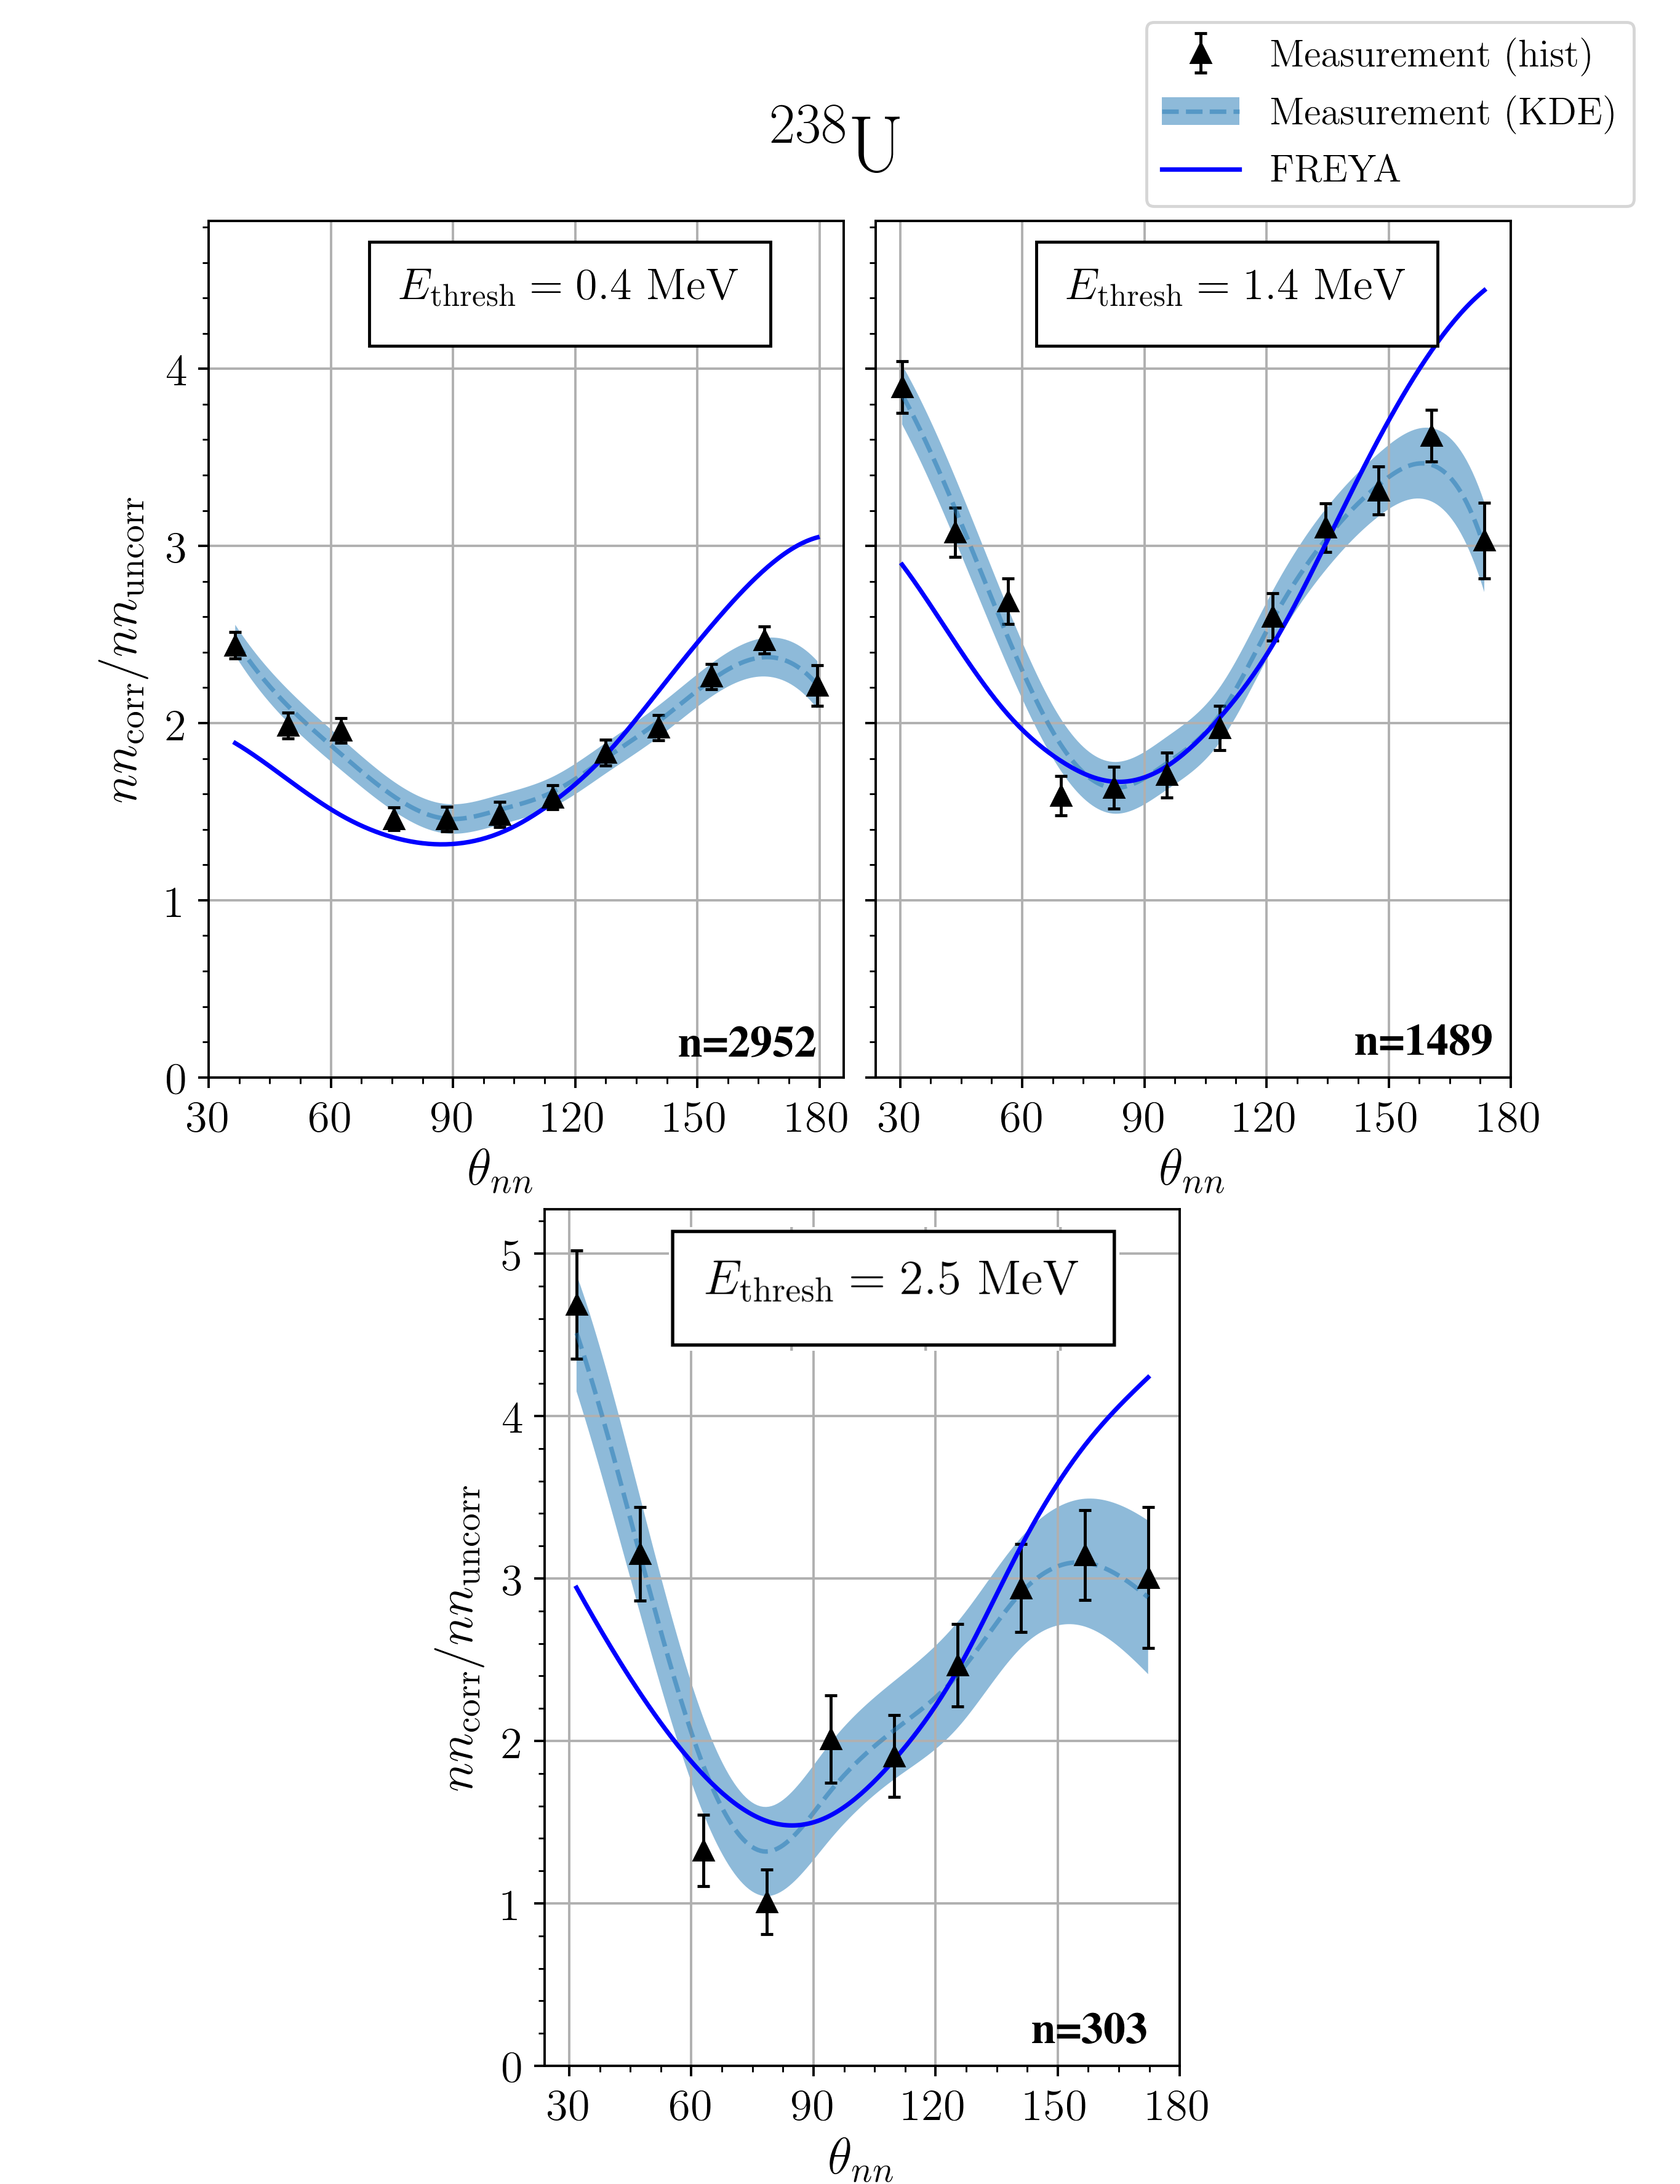
\includegraphics[width = \figsize\textwidth]{FinalDUResultw_freya0(fix)KDE.png}
    \caption{$\theta_{nn}$ distribution with minimum energy threshold cuts applied to all neutrons.
    The number of events contributing to each plot, \textbf{n}, is shown. Note that the bottom plots of this figure and Fig.~\ref{fig:DU(2)} are identical.}
    \label{fig:DU(0)}
\end{figure}
\begin{figure}
\centering
    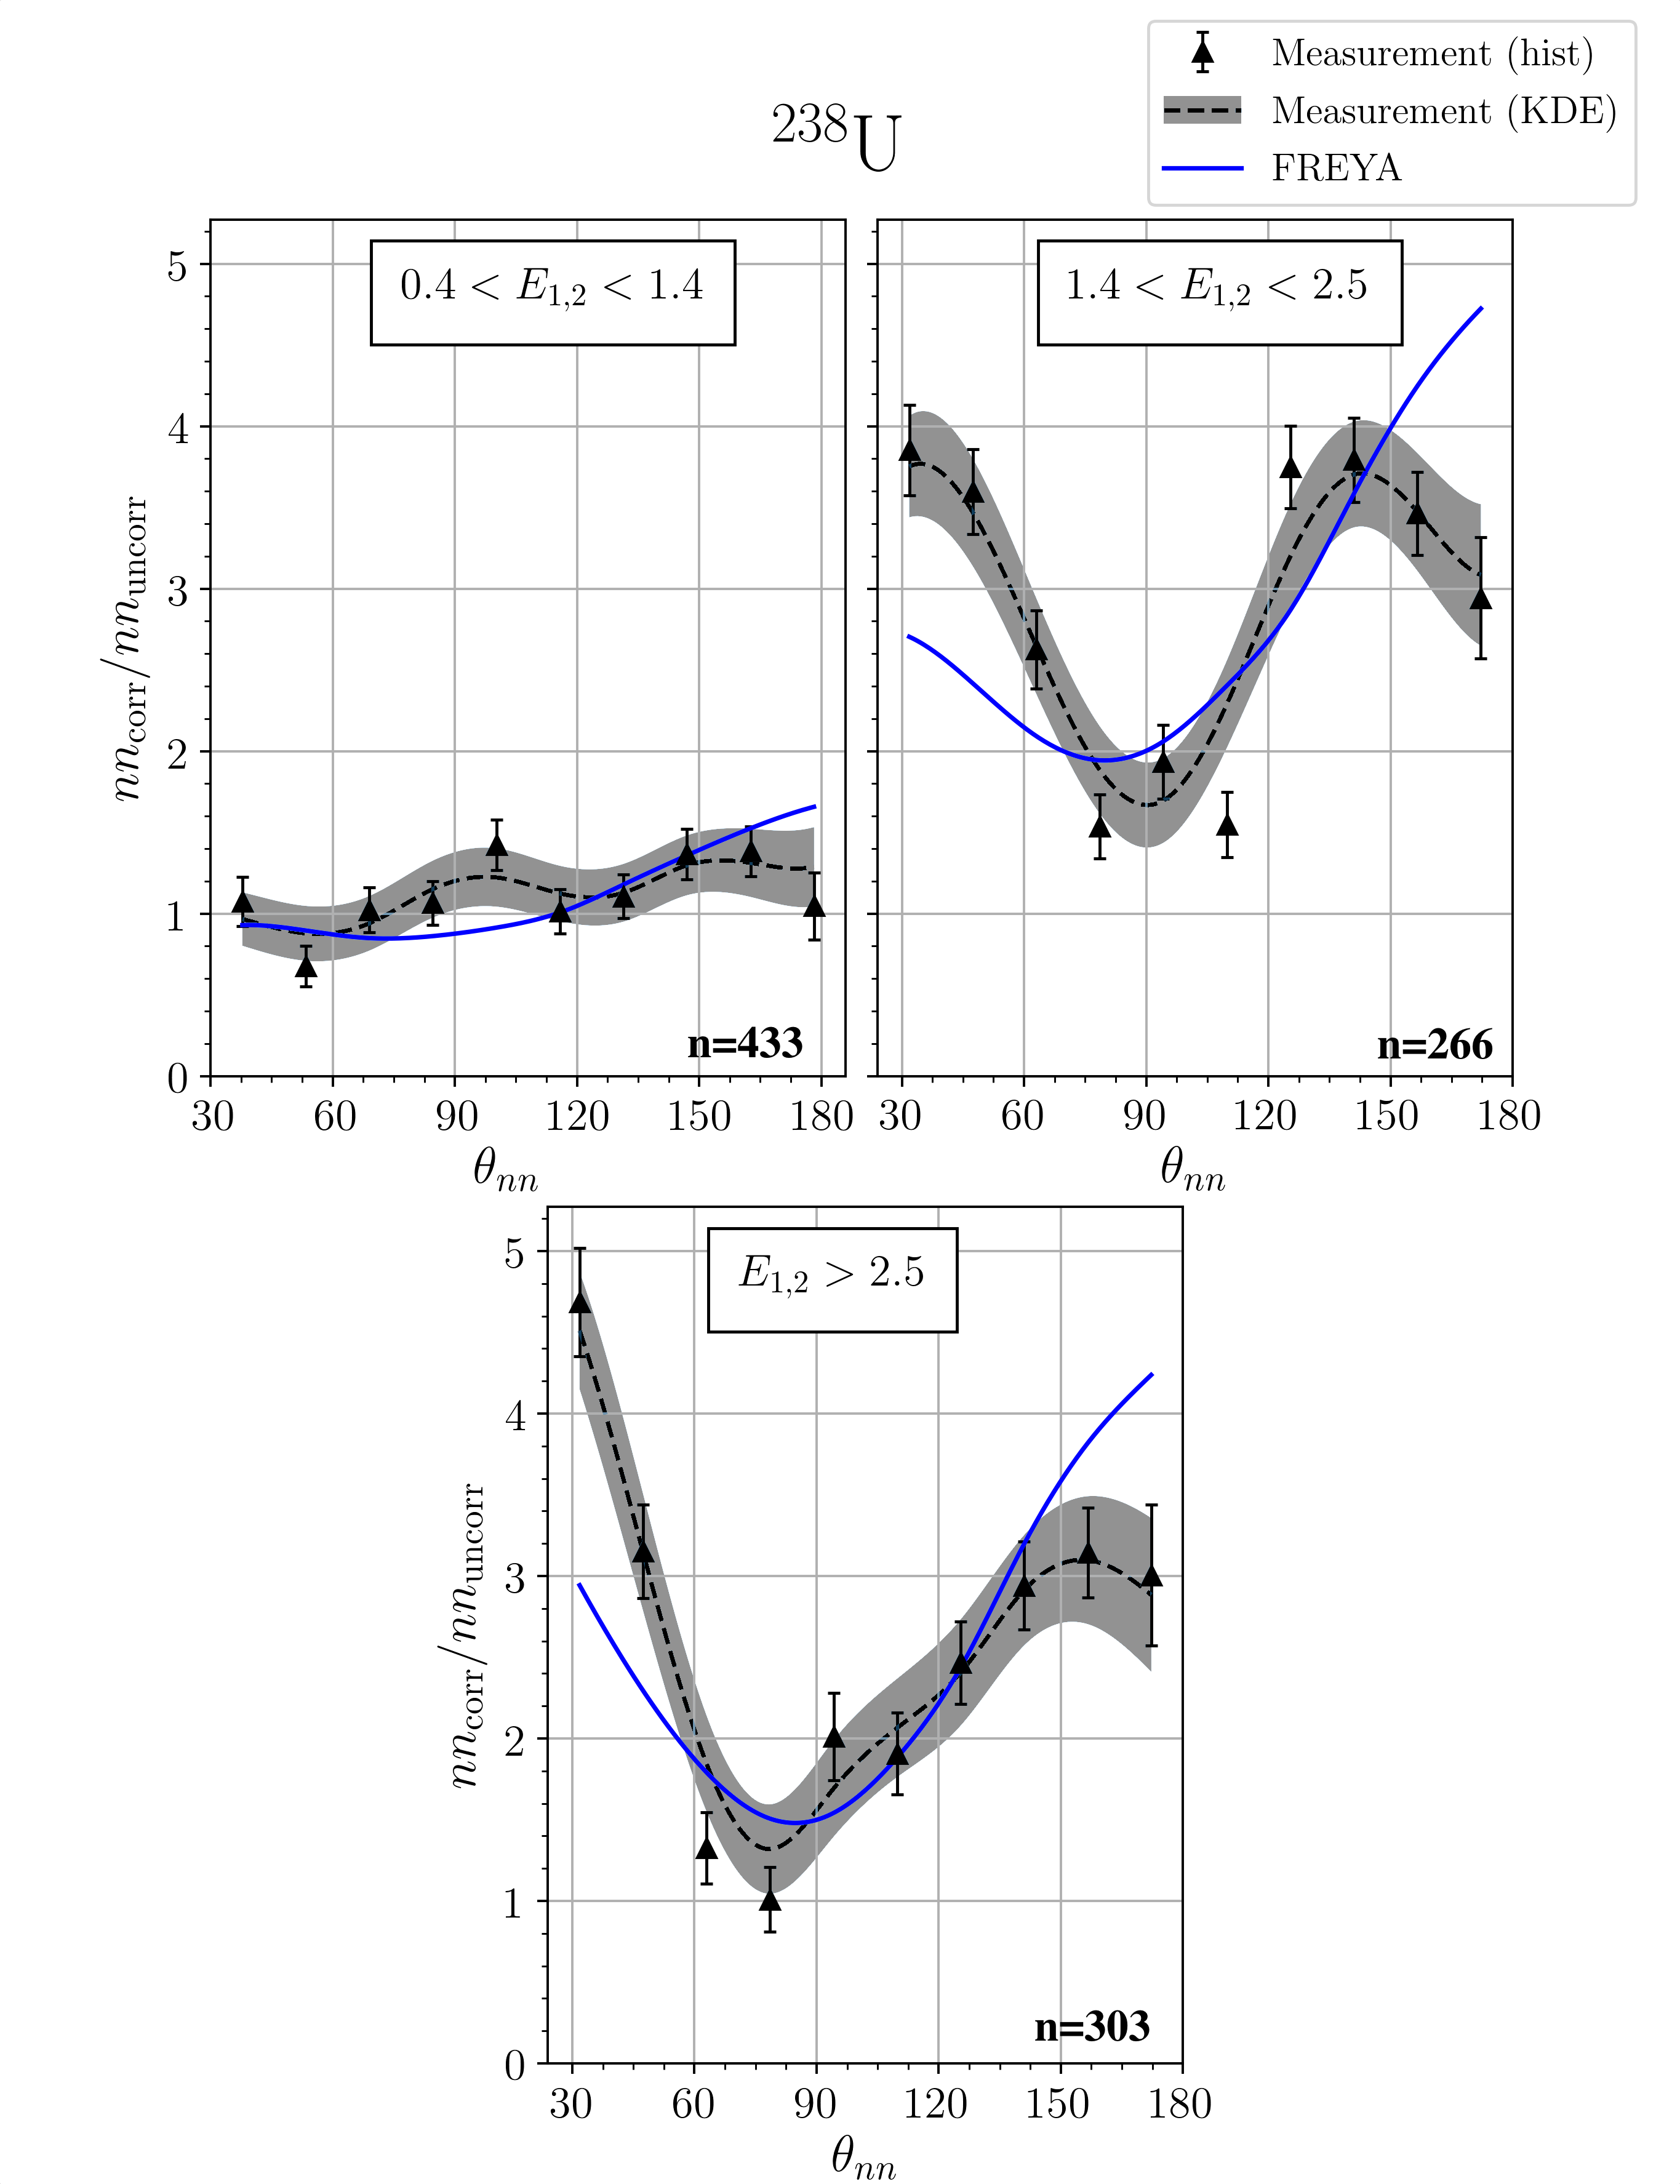
\includegraphics[width = \figsize\textwidth]{FinalDUResultw_freya2KDE(fix).png}
    \caption{ $\theta_{nn}$ distribution with cuts requiring that the energy of both coincident neutrons be within the specified range.
    The number of events contributing to each plot, \textbf{n}, is shown. Note that the bottom plots of this figure and Fig.~\ref{fig:DU(0)} are identical.}
    \label{fig:DU(2)}
\end{figure}

\begin{figure}
\centering
    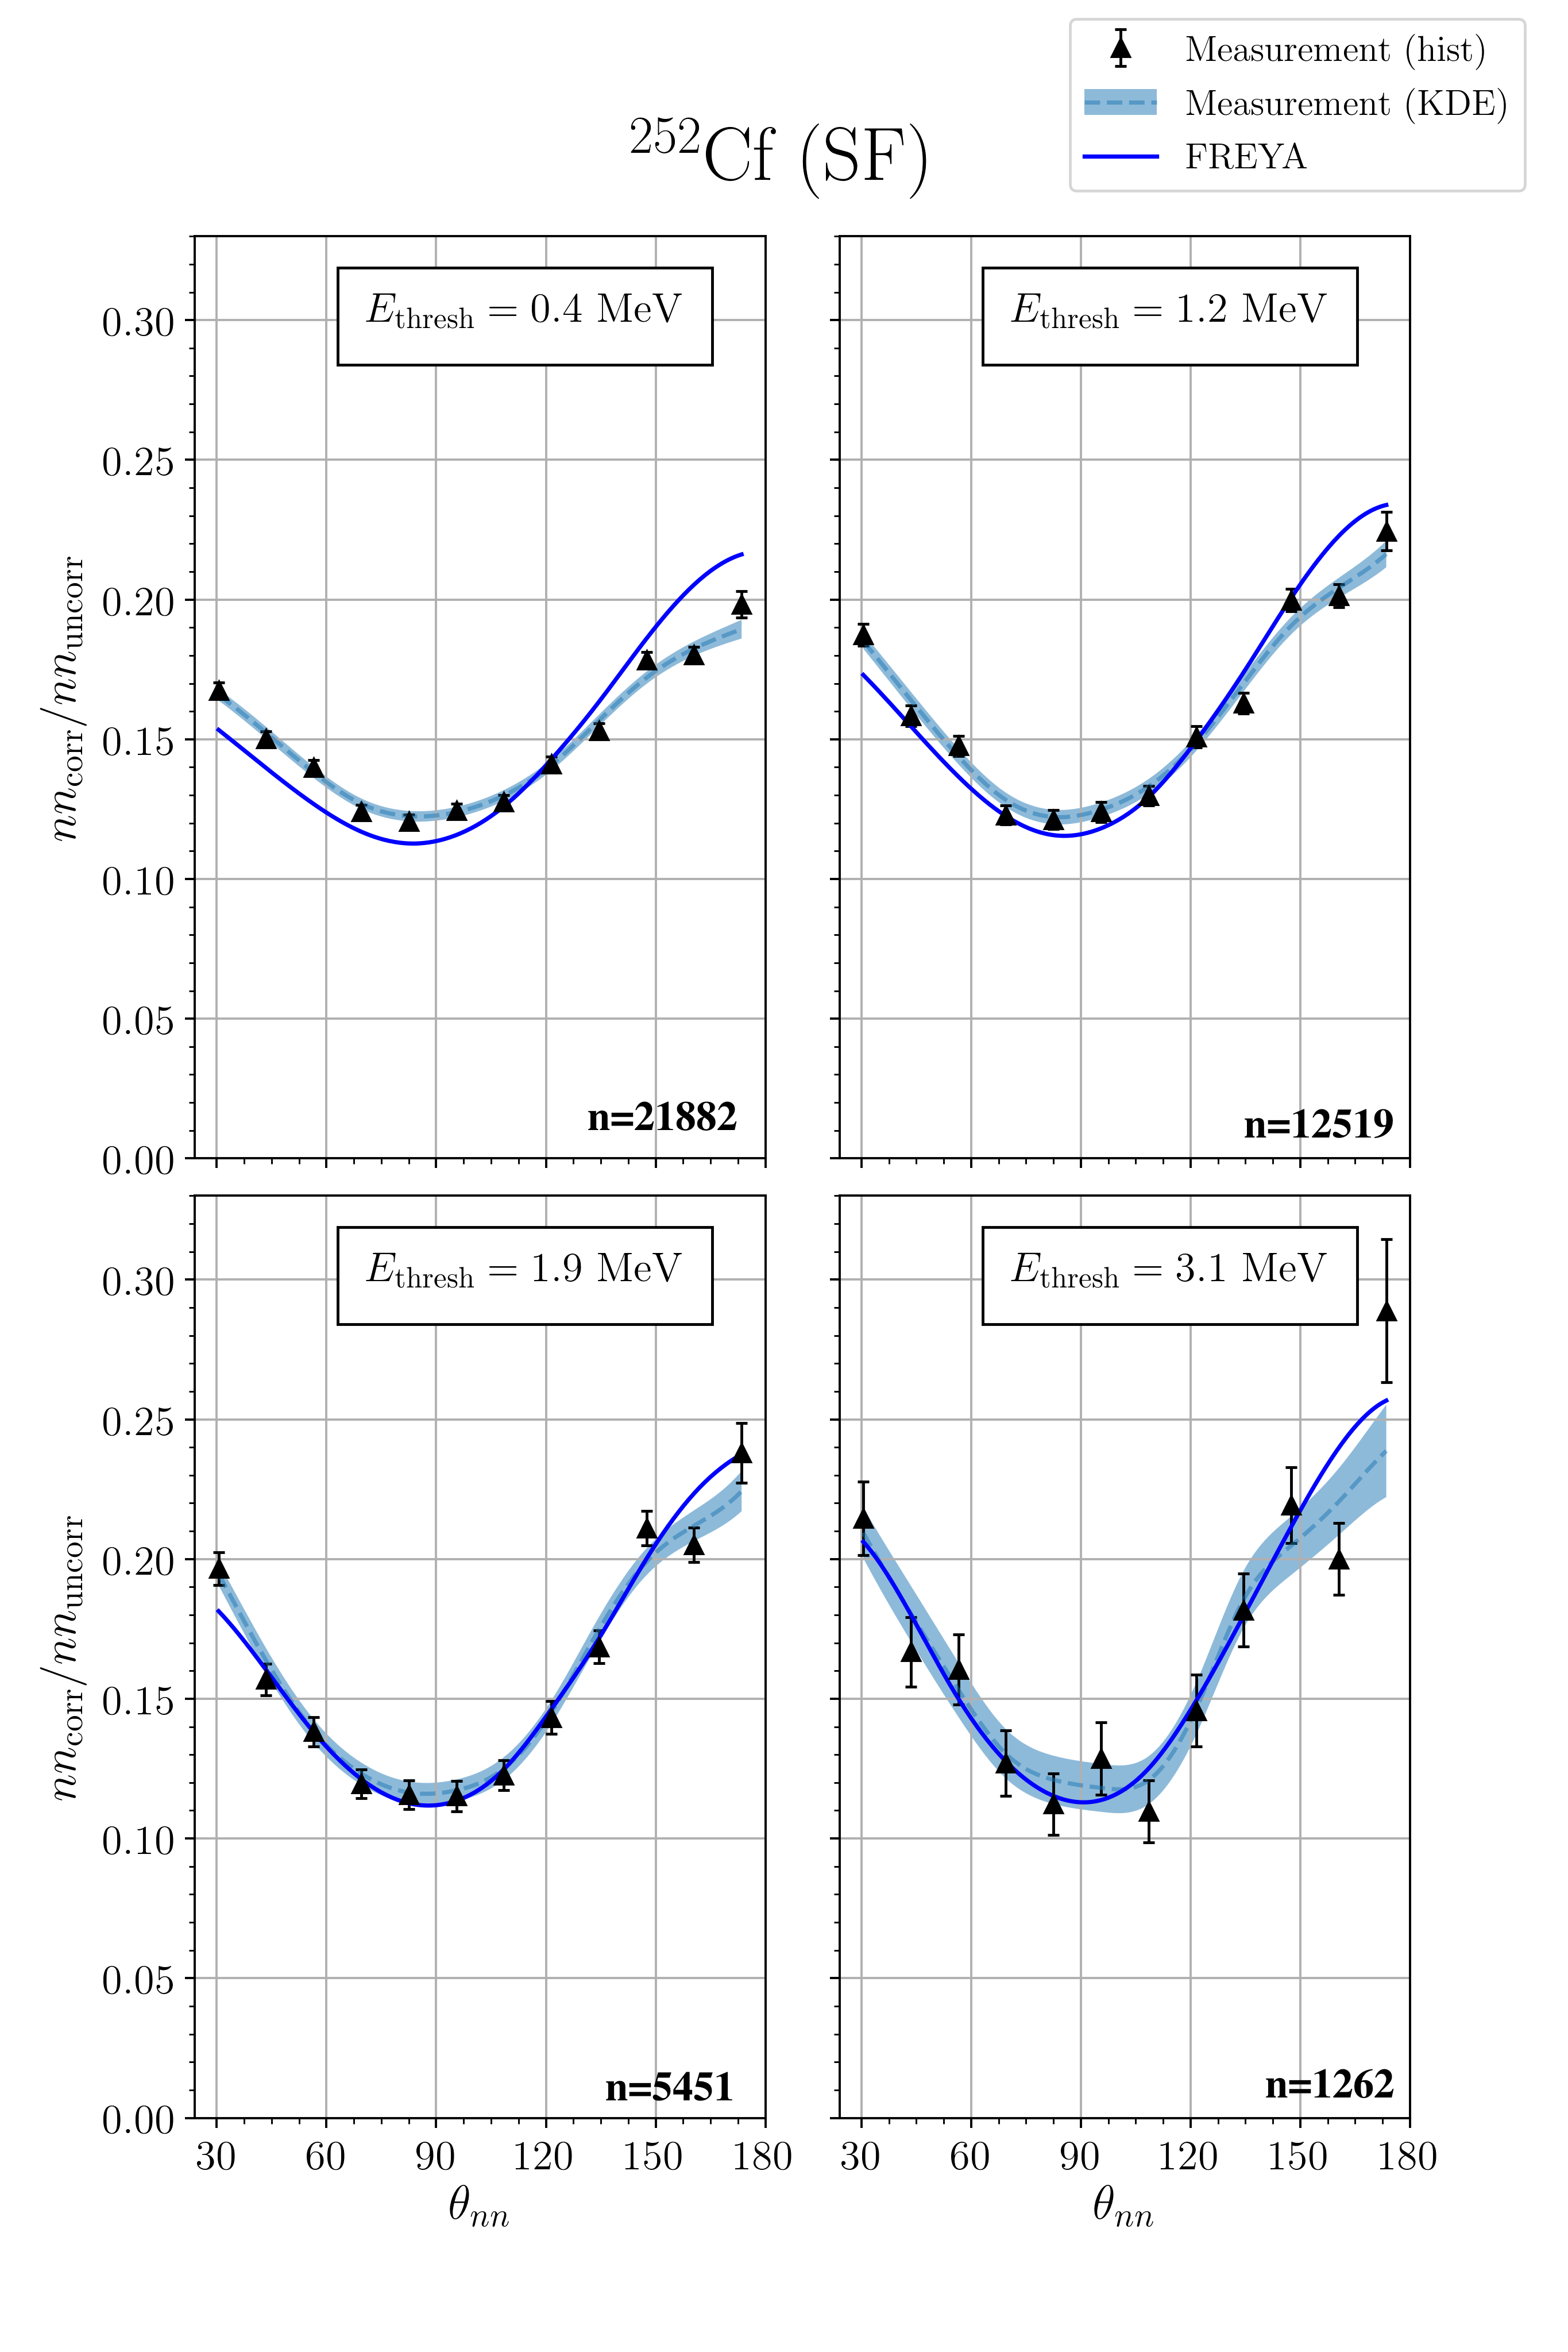
\includegraphics[width = \figsize\textwidth]{FinalCf252Resultw_freya0KDE(fix).png}
    \caption{
    $\theta_{nn}$ distribution a minimum energy threshold cuts applied to all neutrons.
    The number of events contributing to each plot, \textbf{n}, is shown.  Note that the lower right plots of this figure and Fig.~\ref{fig:Cf(2)} are identical.}
    \label{fig:Cf(0)}
\end{figure}
\begin{figure}
\centering
    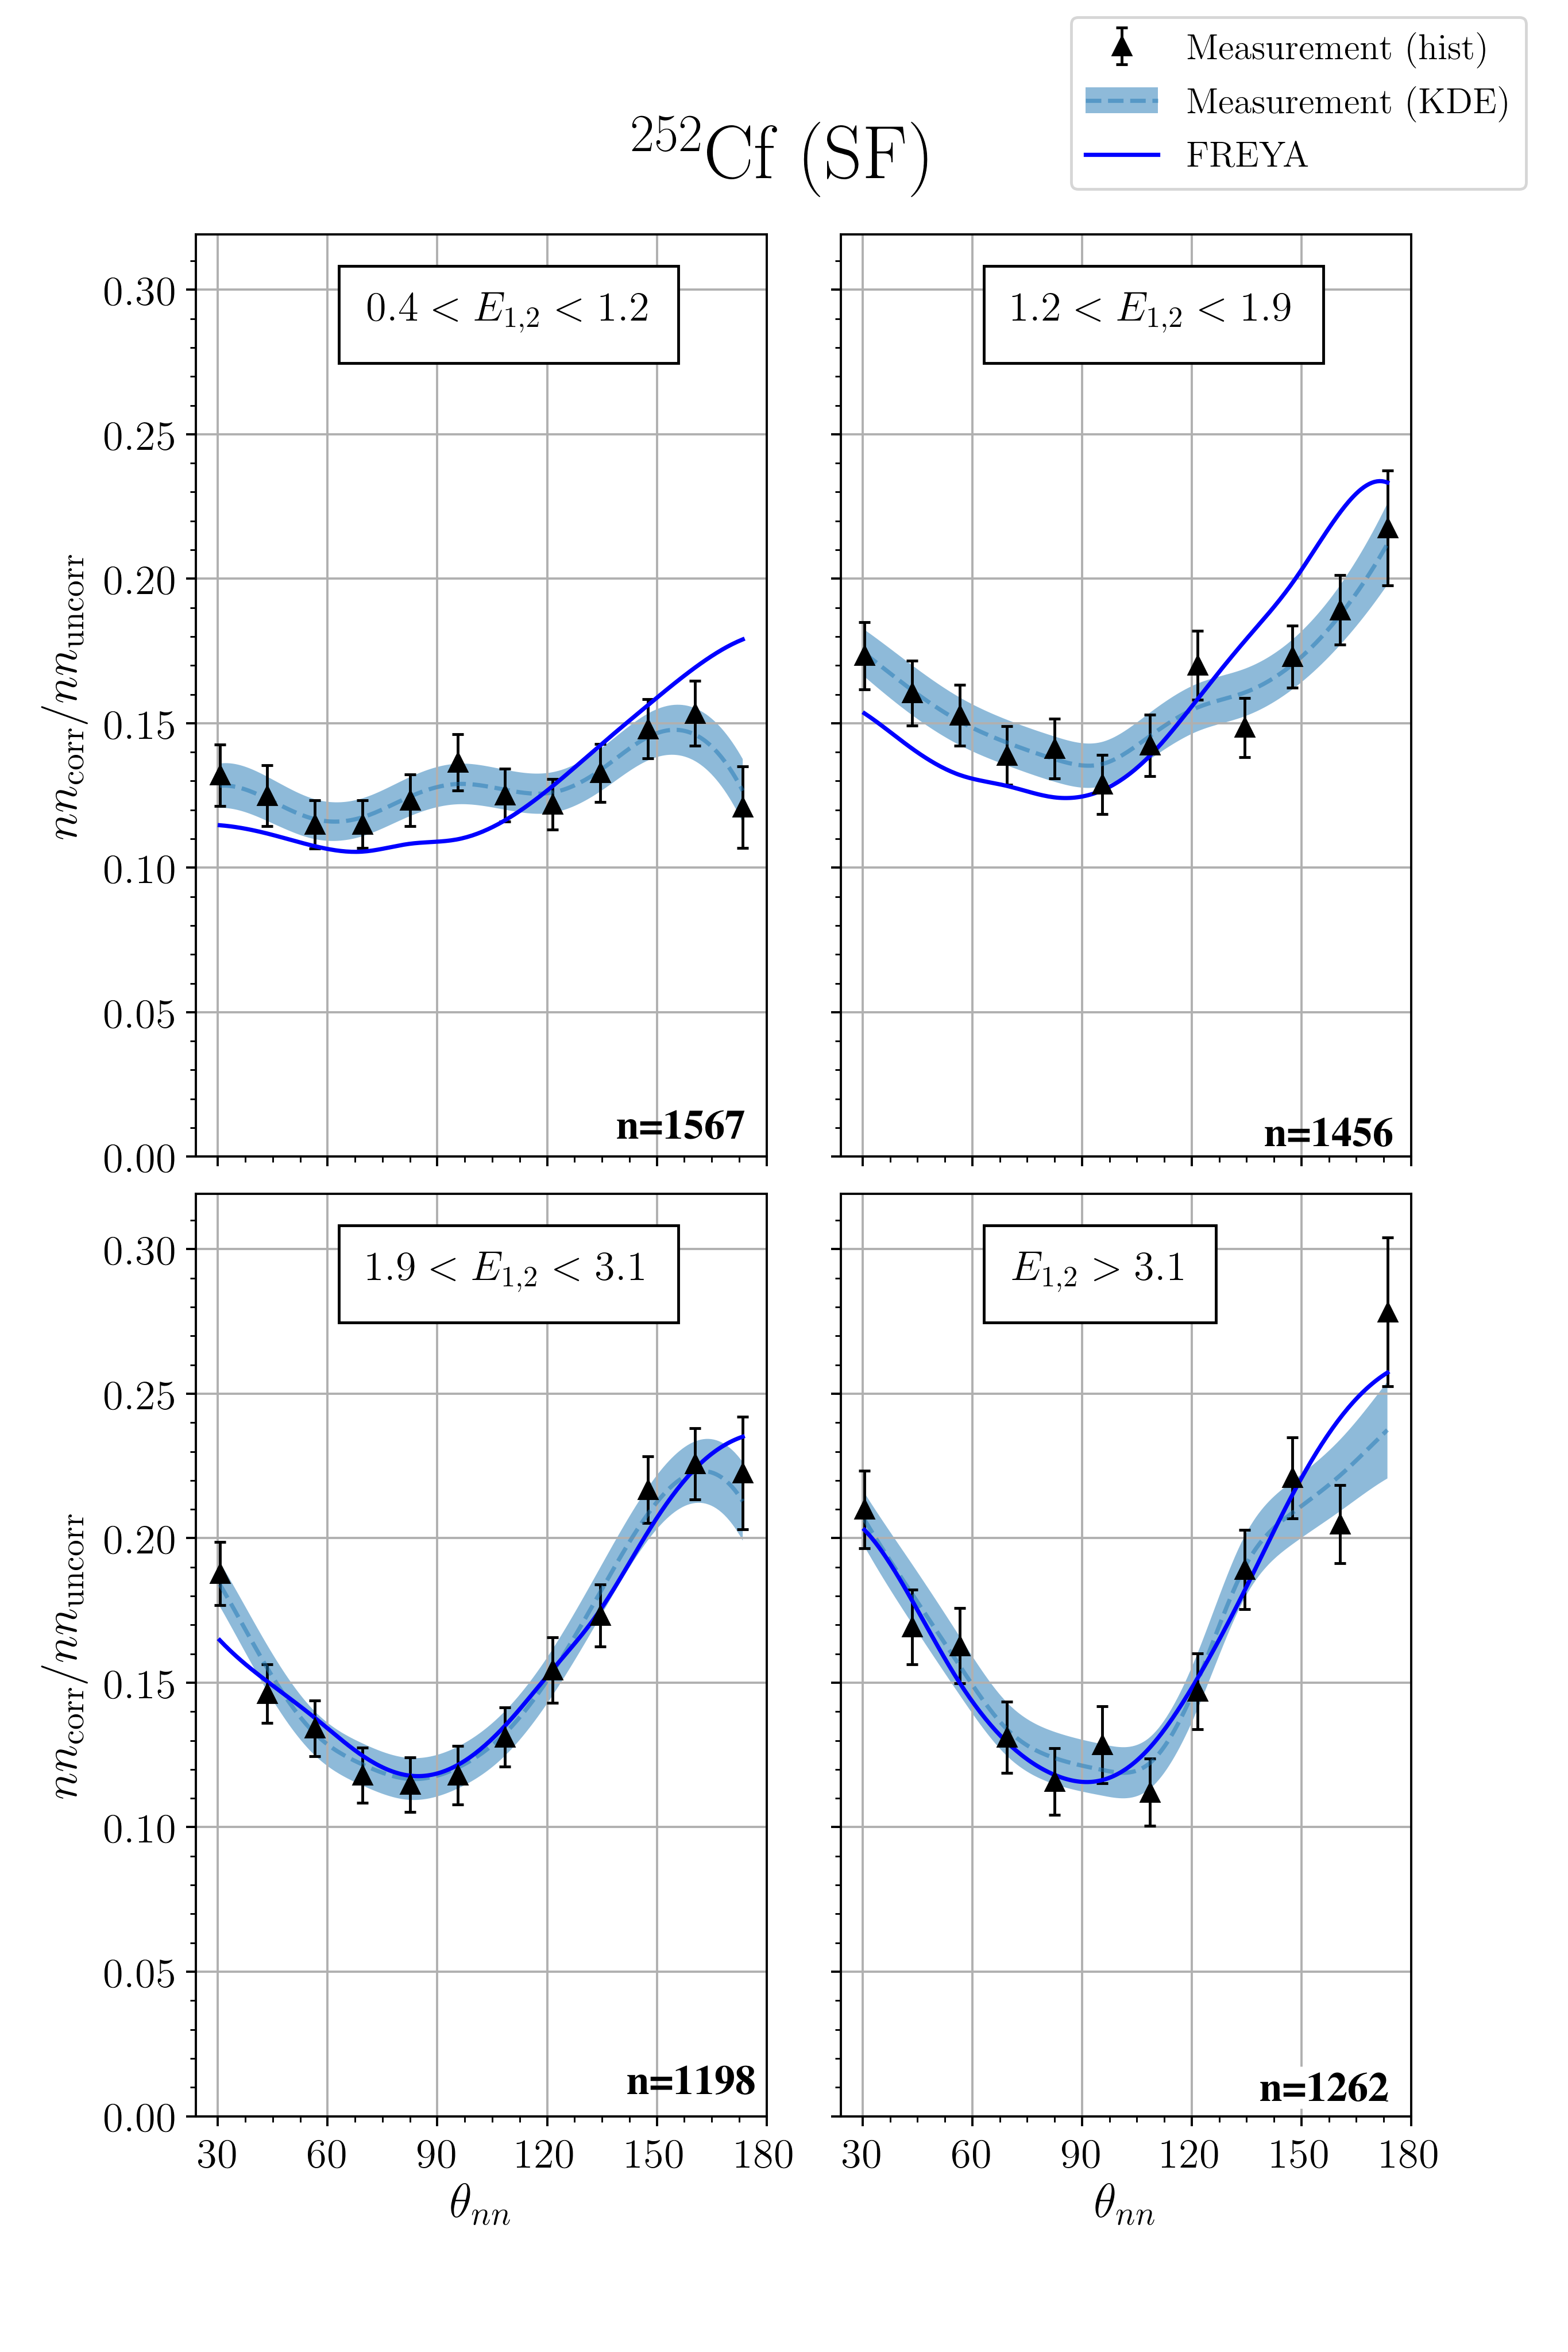
\includegraphics[width = \figsize\textwidth]{FinalCf252Resultw_freya2(fix)KDE.png}
    \caption{$\theta_{nn}$ distribution with cuts requiring that the energy of both coincident neutrons be within the specified range.
    The number of events contributing to each plot, \textbf{n}, is shown. Note that the lower right plots of this figure and Fig.~\ref{fig:Cf(0)} are identical.}
    \label{fig:Cf(2)}
\end{figure}

\subsection{Considering $\theta_{abs}$}
\label{sec:anomaly}
While these results are consistent with the effect of the kinematic focusing of the neutrons due to the recoil of the fission fragments, the data show a small but statistically significant decrease in the n-n opening angle correlation in the region from about 165$^{\circ}$ to 180$^{\circ}$, which can be seen in Figs.~\ref{fig:SPDPNormalization} and ~\ref{fig:theta_abs_two_neutron}, as well as in Figs.~\ref{fig:DU(0)} and \ref{fig:DU(2)}.
This feature is not evident in previous work on spontaneous and neutron induced fission.
The effect is particularly strong for the neutron energy cuts being applied in the upper right plots of both Figs.~\ref{fig:DU(0)} and \ref{fig:DU(2)}.
A comparison of the observed decrease after 160 degrees with the null hypothesis that the true distribution remains constant after 160 degrees yields a p-value of 0.01.
This indicates a 1\% probability of obtaining data as compatible with the above hypothesis as the data we observed.
%which yield p-values of 0.01 under the null hypothesis that the true distribution flattens out around 160$^{\circ}$ and remains flat all the way to 180$^{\circ}$.
A similar effect appears in the results reported in ref~\cite{Sokolov2010} for the thermal neutron-induced fission of $^{233}$U and $^{235}$U, but not for the spontaneous fission of $^{252}$Cf or the neutron-induced fission of $^{239}$Pu.
% (insert in sentance above after the word effect?)  ,although less pronounced than that seen in the present work,)

As previously discussed in section~\ref{sec:level1}, photofission differs from spontaneous and neutron induced fission in that the fission fragments for the photon-induced reaction exhibit an asymmetry in their angle of emission, with the most likely orientation of the fission axis lying perpendicular to the direction of the incident photon.
With this in mind, the following series of angular cuts were made on the data.
Fig.~\ref{fig:theta_abs_LEGO} shows the distributions of absolute opening angles of the n-n events for three different cuts on the value of the n-n opening angle.
For n-n opening angles between 120$^{\circ}$ and 160$^{\circ}$, there is an increased preponderance of both neutrons being emitted around 90$^{\circ}$, consistent with the interpretation of kinematic focusing of neutrons coming from fission fragments which are themselves being emitted preferentially at 90$^{\circ}$.
However, in the opening angle region where the n-n correlation is reduced, from about 160$^{\circ}$ to 180$^{\circ}$, this feature is less prominent.

Furthermore, if one plots the opening angle distributions for the case in which at least one neutron is emitted perpendicular to the incident photon \emph{versus} the case in which neither neutron is emitted perpendicular to the incident photon (Fig.~\ref{fig:theta_abs_two_neutron}), one sees distinct differences.
The fact that there are overall differences is not surprising, because in one case (Fig.~\ref{fig:theta_abs_two_neutron} solid line) at least one neutron preferentially receives a kinematic boost from a fission fragment and in the other case (Fig.~\ref{fig:theta_abs_two_neutron} dotted line) neither neutron does.
However, the fact that the n-n correlation is reduced at 180$^{\circ}$ in opening angle when at least one of the neutrons is emitted along the preferred fission axis is unexpected.
This is a feature which does not seem to appear in either neutron-induced fission, previous measurements on spontaneous fission, or our present measurement on spontaneous fission.
The photofission of the even-even $^{238}$U nucleus seems to be unique in this regard. 
The attribution of this effect to the geometric coverage of the neutron detection system or to neutron elastic scattering within the target was ruled out using simulations, as discussed in section~\ref{subsection:Elastic_scattering}.

These data are consistent with two possible explanations relating to the unique feature of the asymmetric angular emission of fission fragments in photofission.
First, it is possible that there is a decrease in neutron emission along the fission axis.
Second, the neutrons may indeed be emitted isotropically in the rest frame of the fission fragment, but one fragment essentially shadows the neutrons emitted from the other fragment, either through absorption or scattering.
If it is the later case, then this effect has the potential to shed light on the time dependence of neutron emission, since shadowing would likely depend on the fission fragment separation.
A definitive interpretation of this decreased n-n correlation for large opening angles in photo-fission requires further study.

\begin{figure}
    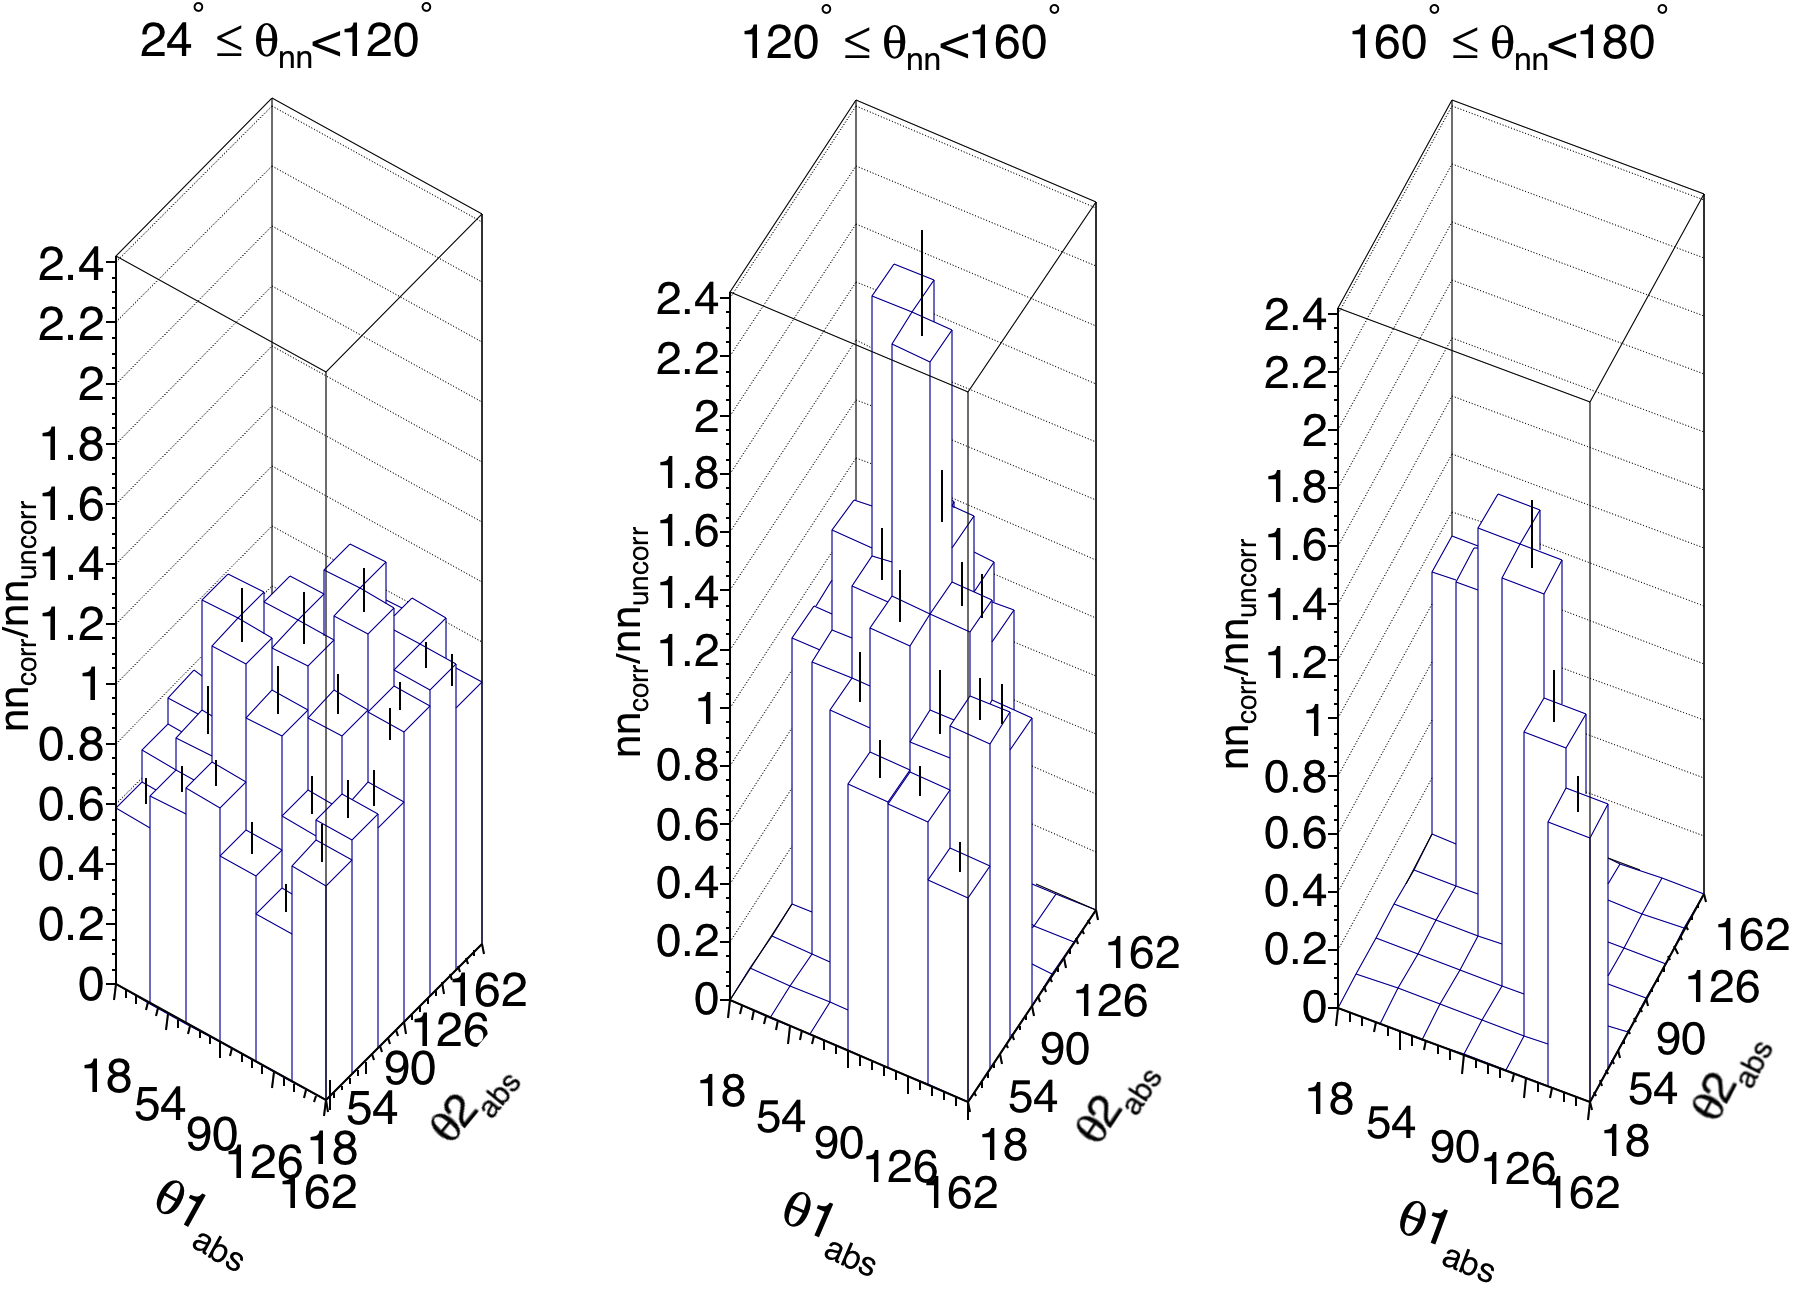
\includegraphics[width = \figsize\textwidth]{theta_abs_LEGO.png}
    \caption{Correlation is shown between the angles of each neutron with respect to the incident photon beam, denoted by $\theta 1_{abs}$ and $\theta 2_{abs}$.
    Empty bins exist because of intrinsic geometrical phase-space.}
    \label{fig:theta_abs_LEGO}
\end{figure}

\begin{figure}
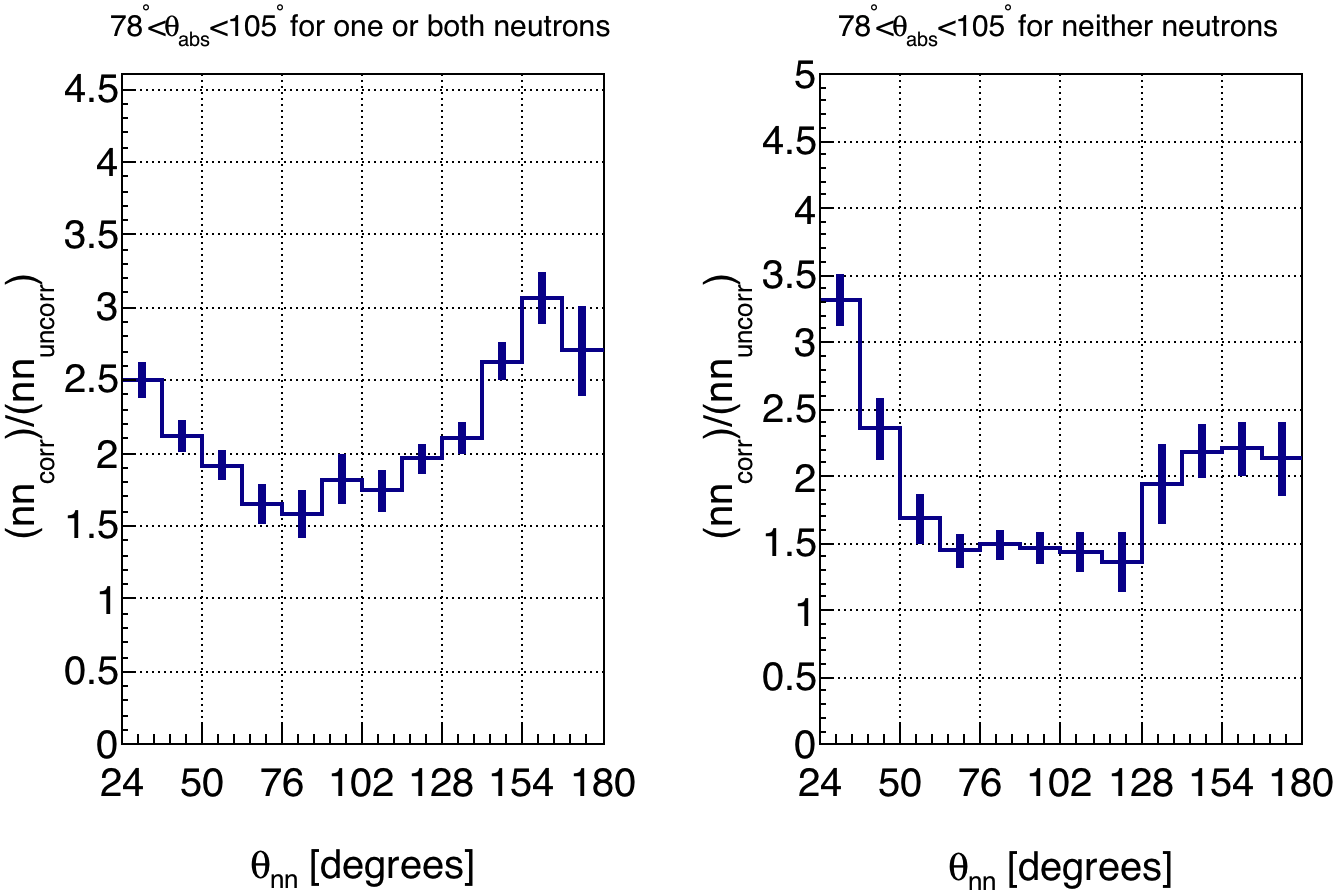
\includegraphics[width=\figsize\textwidth]{theta_abs_two-neutron.png}
\caption{Requiring that at least one of the coincident neutrons be emitted nearly perpendicular to the photon beam (solid line) produces an opening angle distribution that is different from that produced when it is required that both neutrons are emitted nearly parallel to the photon beam (dotted line).}
\label{fig:theta_abs_two_neutron}
\end{figure}